\documentclass[12pt]{article}

\usepackage[fontset=none]{ctex}
\setCJKmainfont{Noto Serif CJK SC}
\setCJKsansfont{Noto Serif CJK SC}
\setCJKmonofont{Noto Sans CJK SC}

\usepackage{graphicx,float,indentfirst,amsmath,amssymb,geometry,subfig,hyperref}

\hypersetup{hidelinks}

\geometry{a4paper,scale=0.8}

\title{霍尔效应}
\author{}
\date{\today}

\begin{document}

\maketitle
\setlength{\parindent}{2em}

\section*{摘要}

霍尔效应具有广泛的运用。本实验通过对霍尔元件参量的测量,了解了霍尔效应的原理及相关参数的测量方式,并掌握了利用霍尔元件测试磁感应强度的办法,并进一步研究了半导体元件的磁电阻效应。

\section{霍尔元件的输出电压与输入电流}

\subsection{原理}
霍尔电压与有关参数有如下关系:$U_H = R_H \frac{IB}{d}=K_H$,其中,$R_H$为霍尔系数,$K_H$为霍尔片的灵敏度。在测量时会产生一些副效应,我们通过测量不同磁场方向和不同电流方向下的B,I来消除副效应。具体的实现方法是测量$U_1(+B,+I)$,$U_2(+B,-I)$,$U_3(-B,-I)$,$U_4(-B,+I)$,可推导:$U_H=\frac{1}{4}(U_1-U_2+U_3-U_4)$。在霍尔元件中,霍尔电压的产生是由于磁场作用下载流子受洛伦兹力作用而迁移,故载流子浓度十分重要。可推导有:$R_H=\frac{1}{ne}$,其中$n$为载流子浓度。

\subsection{实验过程及数据分析}
按原理部分,通过多次改变磁场与电流方向测量来减少副效应的影响。实验进行中,保持激励电流$I_M=500mA$,我们通过开关使电流反向从而达到让磁场和电流反向的效果。测量多组数据,结果见\ref{tab:a1}。根据原理的描述,计算$U_H$并将其与$I$进行线性拟合,结果如下图:

\begin{figure}[H]
    \centering
    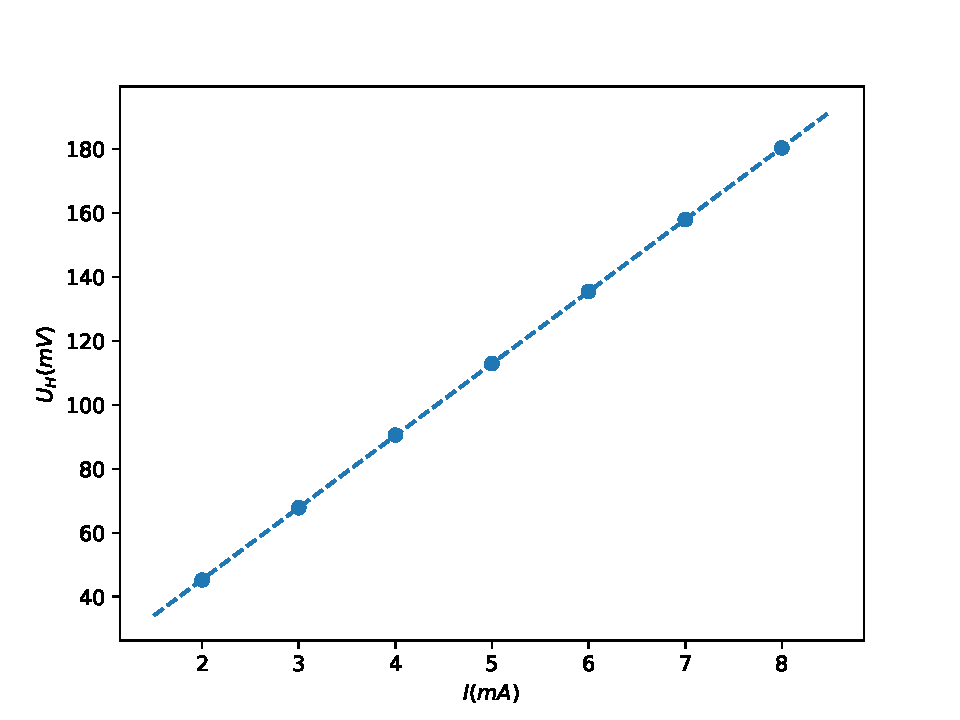
\includegraphics[width=0.7\textwidth]{part1.pdf}
    \label{fig:1}
    \caption{输出电压与输入电流的关系}
\end{figure}

得到斜率为22.514,有标准差0.121。由于本仪器$I_M=500mA$时,$B=127.1mT$。故可计算得到:$K_H=177.138 V \cdot (A \cdot T)^-1$(注:单位为伏每安特斯拉)。进一步进行不确定度分析,认为$B$的不确定度为0,则$K_H$的相对不确定度$U_{K_H}=0.53\%$。根据原理,我们还可以得到霍尔系数$R_H=5.314\times10^{-4} m \cdot V \cdot (A \cdot T)^-1$以及载流子浓度$n=1.174\times10^{22}m^{-3}$。另外,由方向关系可知,霍尔元件的载流子是是电子而不是空穴。

最终我们消除了$U_0$。但是有的时候,我们需要测定不等位效应$U_0$。由于$U_0$源于材料的不均匀等原因,其并不会随着电流或磁场方向反转而反转。故只需要比较正向和反向电流测定的霍尔电压,正向与方向磁场测定的霍尔电压,就可以计算出$U_0$。

\section{激励电流与磁极间磁场的关系}

另外一个重要的关系式是激励电流与磁极间磁场的关系,这是另一种获得磁场的方法。前面我们已经得到了一种测定磁场的方法。我们保持工作电流$I=4.00mA$,改变$I_M$,测定相应的$B$,结果如\ref{tab:a2}。画图,观察到数据呈线性,进行拟合,如下图:

\begin{figure}[H]
    \centering
    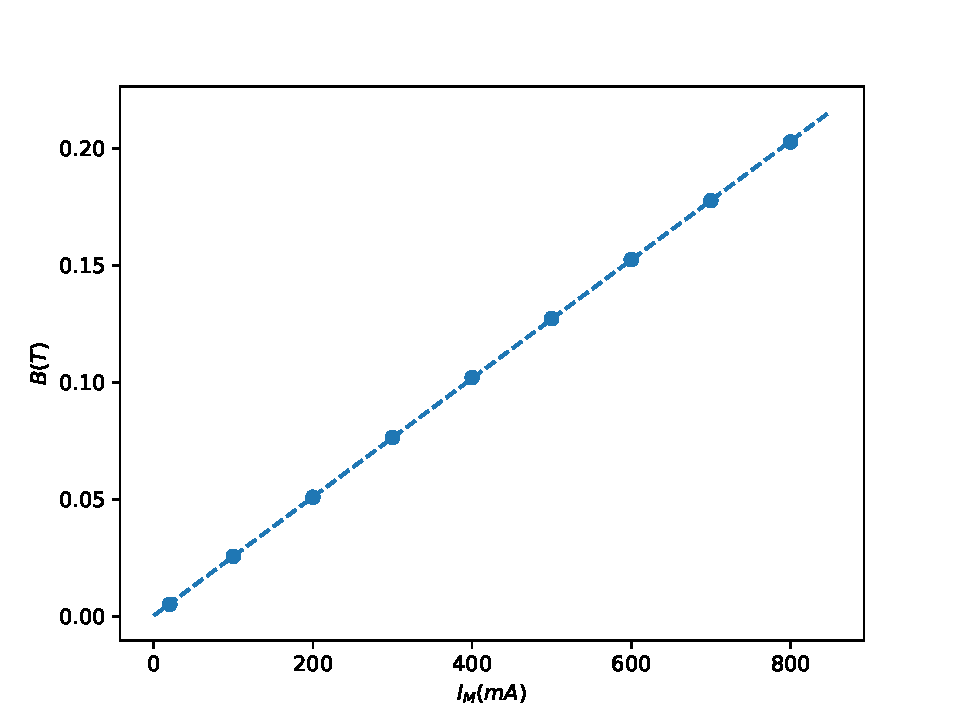
\includegraphics[width=0.7\textwidth]{part3.pdf}
    \label{fig:2}
    \caption{激励电流与磁极间磁场的关系}
\end{figure}

最终结果为斜率$k=0.0002533$,截距为$0.0002971T$,由于磁感应强度的量级在$0.01T$到$0.20T$左右,截距相比起来很小,近似认为截距为零,此时就有关系式:$I=4.00mA$时,$B=0.0002533I_M$(式中$I_M$的单位为mA,$B$的单位为T)。

\section{磁极间隙水平方向磁场的分布曲线}

有了前述的测量磁感应强度的方法,我们可以测量磁极间隙水平方向磁场的分布曲线。保持工作电流$I=4.00mA$,激励电流$I_M=500mA$,不断移动霍尔元件的水平位置,按照上述的方法测量并计算出磁场。测量数据如\ref{tab:a3}。计算后画图,得到下面的磁感应强度分布图:

\begin{figure}[H]
    \centering
    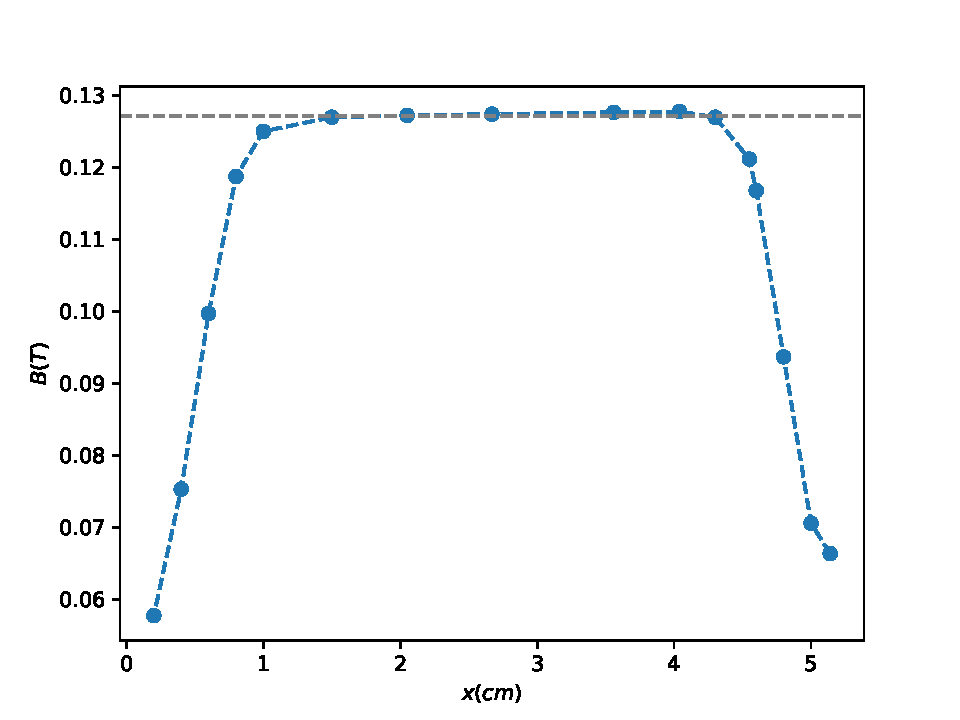
\includegraphics[width=0.7\textwidth]{part5.pdf}
    \label{fig:3}
    \caption{磁极间隙水平方向磁场的分布曲线}
\end{figure}

图中灰色虚线为$I_M=500mA$时实验室给出的磁感应强度。由图可知,磁场在电磁铁中间较为稳定,实验室给出的磁感应强度便是从这里测出来的。在电磁铁的边界处磁感应强度迅速衰减,这是一个很自然的物理图像。

\section{计算载流子迁移率}
\subsection{原理}
载流子在磁场中受到洛仑兹力的作用,在磁场和电场下漂移,形成电流。在电场下,载流子的平均漂移速度v与电场强度E成正比,比例系数就是载流子迁移率。经过推导,有:载流子迁移率$\mu = \frac{K_H I l}{bU}$,其中l沿外加电流方向,b垂直于外加电流与磁场方向。

\subsection{实验过程及数据分析}
与上面类似,进行测量,不过需要测量知道工作电流正向方向的电压。$I=4.00mA$,$I_M=500mA$,工作电流正向方向电压$U=3.005V$。$K_H$采用前面的计算数据,最终带入得到$\mu = 0.7074 kg^{-1}sC$

\section{锑化铟磁阻元件的磁电阻效应}
\subsection{原理}
在一定条件下,导电材料的电阻在外加磁场中发生变化的现象称为磁电阻效应。设磁阻器件在零磁场时电阻及电阻率分别为$R(0)$,$\rho (0)$,磁场为B时电阻及电阻率分别为$R(B)$,$\rho (B)$。通常以电阻率的相对改变量$\Delta \rho / \rho(0)$表示磁阻,$\Delta \rho=\rho(B)−\rho(0)$,而$\Delta R / R(0) \propto \Delta / \rho(0)$,其中$\Delta R=R(B)−R(0)$。为看到磁阻的变化,只需做出$\Delta R / R(0)$与B的关系曲线即可。

\subsection{实验过程及数据分析}
使用锑化铟作为研究对象。其中的AB端短路,CD端外加恒流。为测$R_0$,先空载,电流$I_{CD}=1.50mA$,电压$U=0.5274V$。随后测定不同磁场下的锑化铟电压来计算阻值。通过调控$I_M$调控磁场。(在前面我们已经计算出了$I_M$与$B$的关系式)测量数据如\ref{tab:a4}。画出$\Delta R / R(0)$与B的关系曲线,如下图:

\begin{figure}[H]
    \centering
    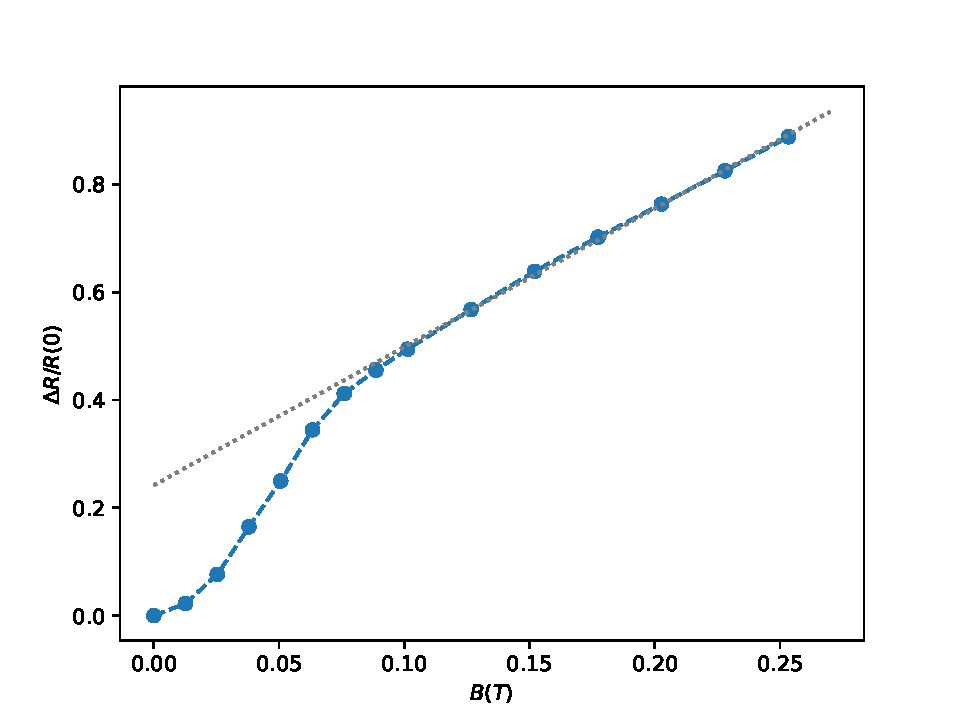
\includegraphics[width=0.7\textwidth]{part4.pdf}
    \label{fig:4}
    \caption{$\Delta R / R(0)$与B的关系曲线}
\end{figure}

可看出,有明显的磁电阻效应。且由线性部分和非线性部分组成。磁场较弱时为非线性区,较强时为线性区。

\clearpage

\appendix
\section{附录}
\renewcommand{\thetable}{附表\arabic{table}}
\setcounter{table}{0}

所有原始数据列在了下面的表格中:(表格内容与电子化原始数据截图一致,故不列出截图)

\begin{table}[H]
    \centering
    \begin{tabular}{|c|c|c|c|c|}
    \hline
    $I(mA)$ & $U_1(mV)$ & $U_2(mV)$ & $U_3(mV)$ & $U_4(mV)$ \\ \hline
    2.00    & 46.0      & -45.9     & 44.6      & -44.5     \\ \hline
    3.00    & 69.1      & -68.9     & 66.8      & -66.6     \\ \hline
    4.00    & 92.3      & -92.0     & 89.2      & -88.8     \\ \hline
    5.00    & 115.2     & -114.7    & 111.3     & -110.7    \\ \hline
    6.00    & 138.2     & -137.6    & 133.5     & -132.8    \\ \hline
    7.00    & 161.2     & -160.3    & 155.6     & -154.6    \\ \hline
    8.00    & 184.1     & -183.0    & 177.8     & -176.5    \\ \hline
    \end{tabular}
    \caption{输出电压与输入电流的关系}
    \label{tab:a1}
\end{table}

\begin{table}[H]
    \centering
    \begin{tabular}{|c|c|c|c|c|}
    \hline
    $I_m(mA)$ & $U_1(mV)$ & $U_2(mV)$ & $U_3(mV)$ & $U_4(mV)$ \\ \hline
    20        & 5.7       & -5.4      & 1.8       & -1.6      \\ \hline
    100       & 19.8      & -19.5     & 16.8      & -16.5     \\ \hline
    200       & 37.6      & -37.3     & 34.8      & -34.5     \\ \hline
    300       & 55.7      & -55.4     & 52.8      & -52.5     \\ \hline
    400       & 73.9      & -73.6     & 71.0      & -70.6     \\ \hline
    500       & 91.6      & -91.3     & 89.0      & -88.6     \\ \hline
    600       & 109.5     & -109.2    & 106.8     & -106.4    \\ \hline
    700       & 127.3     & -127.0    & 124.7     & -124.3    \\ \hline
    800       & 145.1     & -144.7    & 142.5     & -142.0    \\ \hline
    \end{tabular}
    \caption{激励电流与磁极间磁场的关系}
    \label{tab:a2}
\end{table}

\begin{table}[H]
    \centering
    \begin{tabular}{|c|c|c|c|c|}
    \hline
    $x(cm)$ & $U_1(mV)$ & $U_2(mV)$ & $U_3(mV)$ & $U_4(mV)$ \\ \hline
    5.14    & 48.5      & -48.2     & 45.8      & -45.5     \\ \hline
    5.00    & 51.7      & -51.4     & 48.6      & -48.3     \\ \hline
    4.80    & 68.1      & -67.8     & 65.0      & -64.6     \\ \hline
    4.60    & 84.5      & -84.2     & 81.3      & -81.0     \\ \hline
    4.55    & 87.6      & -87.3     & 84.4      & -84.1     \\ \hline
    4.30    & 91.7      & -91.4     & 88.6      & -88.2     \\ \hline
    4.04    & 92.3      & -91.9     & 89.1      & -88.8     \\ \hline
    3.56    & 92.2      & -91.9     & 89.0      & -88.7     \\ \hline
    2.67    & 92.0      & -91.7     & 88.9      & -88.5     \\ \hline
    2.05    & 91.9      & -91.6     & 88.7      & -88.4     \\ \hline
    1.50    & 91.7      & -91.4     & 88.6      & -88.2     \\ \hline
    1.00    & 90.3      & -90.0     & 87.2      & -86.8     \\ \hline
    0.80    & 85.9      & -85.5     & 82.7      & -82.4     \\ \hline
    0.60    & 72.4      & -72.1     & 69.2      & -68.9     \\ \hline
    0.40    & 55.1      & -54.8     & 51.9      & -51.6     \\ \hline
    0.20    & 42.6      & -42.3     & 39.5      & -39.2     \\ \hline
    \end{tabular}
    \caption{磁极间隙水平方向磁场的分布}
    \label{tab:a3}
\end{table}

\begin{table}[H]
    \centering
    \begin{tabular}{|c|c|}
    \hline
    $I_M(mA)$ & $U(V)$ \\ \hline
    50        & 0.5393 \\ \hline
    100       & 0.5677 \\ \hline
    150       & 0.6142 \\ \hline
    200       & 0.6591 \\ \hline
    250       & 0.7091 \\ \hline
    300       & 0.7446 \\ \hline
    350       & 0.7676 \\ \hline
    400       & 0.7881 \\ \hline
    500       & 0.8268 \\ \hline
    600       & 0.8642 \\ \hline
    700       & 0.8977 \\ \hline
    800       & 0.9300 \\ \hline
    900       & 0.9625 \\ \hline
    1000      & 0.9959 \\ \hline
    \end{tabular}
    \caption{$\Delta R / R(0)$与B的关系曲线的测量数据}
    \label{tab:a4}
\end{table}

\end{document}
